\documentclass[a4paper,10pt]{article}
\usepackage[pdftex]{graphicx}
\newcommand{\HRule}{\rule{\linewidth}{0.5mm}}
\usepackage{greektex}
\usepackage{hyperref}
\usepackage{listings}
\usepackage{wrapfig}
\usepackage{graphicx}
\usepackage[usenames,dvipsnames]{color}
\usepackage[table]{xcolor}
\usepackage{colortbl}
%--------Footers-Headers---------------
\usepackage{fancyhdr}
\pagestyle{fancy}
\fancyhead[LE,RO]{\slshape \rightmark}
\fancyhead[LO,RE]{\slshape \leftmark}
\fancyfoot[C]{\thepage}
%-----Greek language-----------------
\usepackage[cm-default]{fontspec}
\usepackage{xunicode}
\usepackage{xltxtra}
\usepackage{amsmath}
\usepackage{xgreek}
%-----Fonts-------------------------
\setromanfont{FreeSerif}
\setsansfont{FreeSans}
\setmonofont{FreeMono}
%----------Hyper linking setup----------------
\hypersetup{
    bookmarks=false,         % show bookmarks bar?
    unicode=true,          % non-Latin characters in Acrobat’s bookmarks
    pdftoolbar=false,        % show Acrobat’s toolbar?
    pdfmenubar=false,        % show Acrobat’s menu?
    pdffitwindow=false,     % window fit to page when opened
    pdfstartview={FitH},    % fits the width of the page to the window
    pdftitle={My title},    % title
    pdfauthor={Author},     % author
    pdfsubject={Subject},   % subject of the document
    pdfcreator={Creator},   % creator of the document
    pdfproducer={Producer}, % producer of the document
    pdfkeywords={keyword1} {key2} {key3}, % list of keywords
    pdfnewwindow=true,      % links in new window
    colorlinks=true,       % false: boxed links; true: colored links
    linkcolor=black,          % color of internal links
    citecolor=green,        % color of links to bibliography
    filecolor=magenta,      % color of file links
    urlcolor=blue           % color of external links
}
%----------code setup----------------
\lstset{language=verilog,
   keywords={module,initial,forever,begin,wait,case,else,elseif,end,for,function,
      if,assign,while,always,or,posedge,endmodule},
   keywordstyle=\bfseries\color{BrickRed},
   keywords=[2]{wire,input,output,reg},
   keywordstyle={[2]\bfseries\color{OliveGreen}},
   basicstyle=\footnotesize,
   commentstyle=\color{blue},
   stringstyle=\color{green},
   numbers=left,
   numberstyle=\tiny\color{black},
   stepnumber=1,
   numbersep=5pt,
   backgroundcolor=\color{Goldenrod},
   tabsize=5,
   showspaces=false,
   frame=single,
   showtabs=false,
   showstringspaces=false} 

%---------image border--------
\usepackage{float}
\floatstyle{boxed} 
\restylefloat{figure}

%---------Figures numbering by section--------
\usepackage{amsmath}
\numberwithin{figure}{subsection}
\numberwithin{table}{subsection}


%opening
%\title{\bf ΛΟΓΙΚΗ ΣΧΕΔΙΑΣΗ 2}
%\author{  Καλάργαρης Χαράλαμποs, AM:3929 \and  Καλάργαρης Χαράλαμποs, AM:3929 \and   Καλάργαρης Χαράλαμποs, AM:3929 }
%\date{27/5/2011}

\begin{document}
\begin{titlepage}

\begin{center}


% Upper part of the page

\includegraphics[width=0.25\textwidth]{/home/federico/Documents/Kile/Diploma/Front_Page/ceid.png}\\[1cm]    
%%/home/federico/Pictures/appmakr-logo.png
\textsc{\LARGE Πανεπιστημίο Πατρών}\\[1.5cm]

\textsc{\Large Μηχανικών Η/Υ και Πληροφορικής}\\[2.5cm]


% Title
\HRule \\[0.4cm]
{ \Large \bfseries Σχεδιασμός System-on-Chip για επεξεργασία εικόνας και υλοποίηση με FPGA. }\\[0.4cm]

\HRule \\[3.5cm]

% Author and supervisor
\begin{minipage}{0.4\textwidth}
\begin{flushleft} \large
\emph{Author:}\\
Χαράλαμπος \textsc{Καλάργαρης}
\end{flushleft}
\end{minipage}
\begin{minipage}{0.4\textwidth}
\begin{flushright} \large
\emph{Supervisor:} \\
Θεμιστοκλής \textsc{Χανιωτάκης}
\end{flushright}
\end{minipage}

\vfill

% Bottom of the page
{\large \today}

\end{center}

\end{titlepage}
%\maketitle
\newpage
\tableofcontents
\newpage
\listoffigures
\newpage
\listoftables
\newpage

\section{Εισαγωγή}
{


}

\newpage
\section{OpenRISC 1200 IP Core}
{
\subsection{Εισαγωγή}

\subsubsection{OpenRISC Οικογένεια}
Η OpenRISC 1000 οικογένεια επεξεργαστών αναφέρεται σε μια ελεύθερη, ανοιχτού
λογισμικού RISC αρχιτεκτονική κεντρικών μονάδων επεξεργασίας.Σχετικά με την
αρχιτεκτονική, η OpenRISC 1000 οικογένεια στοχεύει σε ένα φάσμα υλοποιήσεων που	
ποικίλουν ως προς την τιμή/αποδοση και το είδος της εφαρμογής.Είναι μια 
32/64-bit φόρτωσης και αποθήκευσης (load and store) RISC αρχιτεκτονική που σχεδιάστηκε
με έμφαση στην απόδοση, στην απλότητα, στην χαμηλή ενεργειακή κατανάλωση, στην επεκτασιμότητα
και στην ευελιξία.Η OpenRISC αρχιτεκτονίκη στοχεύει σε μεσσαία και υψηλή απόδοση
δικτύωσης (networking), σε ενσωματομένα, αυτοκινητοβιομηχανικά και φορητά υπολογιστηκά περιβάλλοντα.

\vspace{0.7cm}
\begin{figure}[h!]
 \centering
 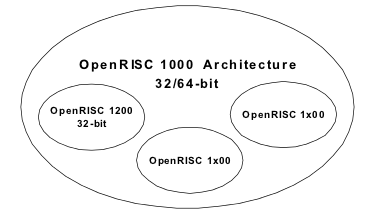
\includegraphics[bb=0 0 376 214,scale=0.7]{/home/federico/Documents/Kile/Diploma/Images/OR_family.png}
 % OR_family.png: 376x214 pixel, 72dpi, 13.26x7.55 cm, bb=0 0 376 214
 \caption{Σχηματική αναπαράσταση OpenRISC αρχιτεκτονικής.}
\end{figure}
\vspace{0.7cm}


Όλες οι OpenRISC υλοποιήσεις που το πρώτο ψηφίο στον αριθμό ταυτότητας
(identification number) ειναι '1' ανήκουν στην 
OpenRISC 1000 οικογένεια.Το δεύτερο ψηφίο ορίζει ποια χαρακτηριστικά της OpenRISC
1000 αρχιτεκτονικής είναι υλοποιημένα και με ποιο τρόπο είναι υλοποιημένα.Τα δύο
τελευταία ψηφία αναφέρονται στο πως μια υλοποίηση ηταν παραμετροποιημένη πριν 
χρησιμοποιηθει σε πραγματική εφαρμογή.

\subsubsection{OpenRISC 1200}
 Ο OR1200 είναι ενας 32-bit βαθμωτός RISC επεξεργαστής με Harvard μικροαρχιτεκτονική,
5 stage integer pipeline, υποστήριξη εικονικής μνήμης (MMU) και βασικές δυνατότητες
DSP.

Οι προκαθορισμένες κρυφες μνήμες ειναι:
\begin{itemize}
 \item 1-way direct-mapped 8KB κρυφή μνήμη δεδομένων.
 \item 1-way direct-mapped 8KB κρυφή μνήμη εντόλων.
 \item Κάθε κρυφή μνήμη έχει γραμμή μεγέθους 16-byte.
 \item Και οι δύο κρύφές μνήμες ειναι  physically tagged(todo).
\end{itemize}

Η προκαθορισμένη MMU αποτελείται από:
\begin{itemize}
 \item 64-entry hash based 1-way direct-mapped data TLB.
 \item 64-entry hash based 1-way direct-mapped instruction TLB.
\end{itemize}

Μερικές άλλες επιπρόσθετες λειτουργίες που παρέχει ο OpenRISC 1200 ειναι η μονάδα
απασφαλμάτωσης πραγματικού χρόνου (real-time debug unit), υψηλής ανάλυσης χρονιστή,
προγραμματιζόμενο ελεκτή διακοπών (programmable interrupt controller) και μονάδα
ρύθμισης των ενεργειακών απαιτήσεων.


Ο OR1200 ουσιαστικά προορίζεται για εφαρμογες σε ενσωματομένα,φορητά και δικτύωσης
συστήματα.Μπορεί να ανταγωνιστεί τους τελευταίους βαθμωτούς 32-bit RISC επεξεργαστές
της κλάσης του και να υποστηρίξει αποδοτικά οποιοδήποτε μοντέρνο λειτουργικό σύστημα.
Ανταγωνιστές του θεωρούνται οι ARM10, ARC και Tensilica RISC επεξεργαστές.
\newline
Συνοπτικά παρουσιάζονται παρακάτω τα χαρακτηριστικά του OR1200:


{%
\newcommand{\mc}[3]{\multicolumn{#1}{#2}{#3}}
\definecolor{tcD}{rgb}{0.968627,0.968627,0.968627}
\definecolor{tcA}{rgb}{1,1,0}
\definecolor{tcB}{rgb}{0.968627,0.968627,0.968627}
\definecolor{tcC}{rgb}{1,1,0.772549}
\begin{table}
\begin{center}
\begin{tabular}{ll}
% use packages: color,colortbl
\rowcolor{tcA}
  & \textbf{OR 1200}\\
\rowcolor{tcD}
\textbf{License} & \textit{GNU LGPL}\\
\rowcolor{tcC}
\textbf{Platform} & \textit{FPGA, ASIC}\\
\mc{1}{>{\columncolor{tcB}}l}{\textbf{Distributed file format}} & \mc{1}{>{\columncolor{tcD}}l}{\textit{Verilog}}\\
\rowcolor{tcC}
\textbf{General} &  \\
\rowcolor{tcD}
Architecture & \textit{32-bit RISC}\\
\rowcolor{tcC}
Byte Ordering & \textit{Big endian}\\
\rowcolor{tcD}
Pipeline depth & \textit{5}\\
\rowcolor{tcC}
Issue type & \textit{Single}\\
\rowcolor{tcD}
\textbf{Register file} &  \\
\rowcolor{tcC}
Organization & \textit{Flat}\\
\rowcolor{tcD}
\# of global registers & \textit{32}\\
\rowcolor{tcC}
Total \# of GPRs & \textit{32}\\
\rowcolor{tcD}
\textbf{ISA} &  \\
\rowcolor{tcC}
Type & \textit{ORBIS32}\\
\rowcolor{tcD}
Addressing modes & \textit{Immediate,
displacement, pcrelative}\\
\rowcolor{tcC}
MAC & \textit{32x32-bit, 48-bit Acc}\\
\rowcolor{tcD}
Custom instructions & \textit{Yes}\\
\rowcolor{tcC}
Custom coprocessor & \textit{Yes}\\
\rowcolor{tcD}
Software floating-point support & \textit{IEEE-754 Single and double precision}\\
\rowcolor{tcC}
\textbf{Cache} &  \\
\rowcolor{tcD}
Hierarchy & \textit{Harvard}\\
\rowcolor{tcC}
Instruction cache
size & \textit{512 byte-8 Kbyte}\\
\rowcolor{tcD}
Data cache size & \textit{4-8 Kbyte}\\
\rowcolor{tcC}
Line size & \textit{8-16 byte}\\
\rowcolor{tcD}
Placement scheme & \textit{Direct-mapped}\\
\rowcolor{tcC}
Valid bits & \textit{One per cache line}\\
\rowcolor{tcD}
Line-locking & \textit{Set basis}\\
\rowcolor{tcC}
\textbf{System Interface} & \textit{Wishbone SoC rev. B32-bit}\\
\rowcolor{tcD}
\textbf{Power Management} & \textit{Slow and idle mode, sleep mode, doze mode}\\
\rowcolor{tcC}
\textbf{Memory} &  \\
\rowcolor{tcD}
On-chip RAM & \textit{Configurable} \\
\rowcolor{tcC}
\textbf{Operating system
support} & \textit{Linux, uClinux, OAR RTEMS RTOS}\\
\end{tabular}
\end{center}
\caption{Overview of OR1200 specifications}
\end{table}
}%
\vspace{0.7cm}
\newpage


\subsection{Αρχιτεκτονική}
Στο παρακάτω σχήμα βρίσκεται η σχηματική αναπαράσταση του OR1200 επεξεργαστή όπου αποτελείται από τις εξής υπομονάδες:
\begin{itemize}
 \item CPU/FPU/DSP central block.
 \item Direct-mapped data cache.
 \item Direct-mapped instruction cache.
 \item Data MMU based on hash based DTLB.
 \item Instruction MMU based on hash based ITLB.
 \item Power management unit and power management interface.
 \item Tick timer.
 \item Debug unit and development interface.
 \item Interrupt controller and interrupt interface.
 \item Instruction and Data WISHBONE host interfaces.
\end{itemize}
\begin{figure}[h!]
 \centering
 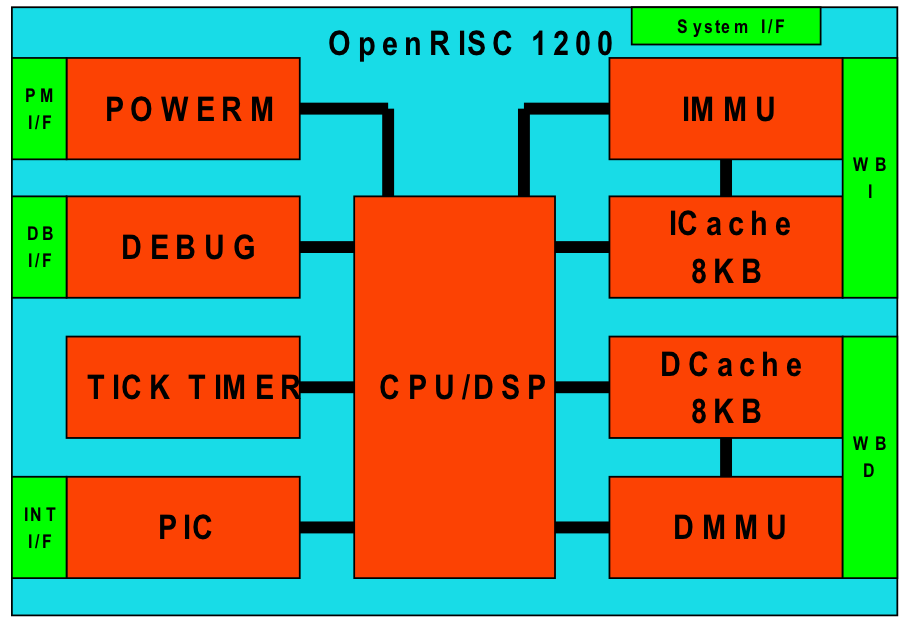
\includegraphics[bb=0 0 905 625,scale=0.3]{/home/federico/Documents/Kile/Diploma/Images/or1200.png}
 % or1200.png: 905x625 pixel, 72dpi, 31.93x22.05 cm, bb=0 0 905 625
 \caption{Core's Architecture}
\end{figure}

\subsubsection{CPU/DSP}
Το μπλόκ CPU/FPU/DSP είναι ένα κεντρικό κομμάτι του επεξεργαστή OR1200 RISC. Το σχήμα 2.3 δείχνει
το βασικό μπλόκ διάγραμμα του CPU/DSP (δεν απεικονίζεται η μονάδα FPU). Η μονάδα του OR1200 CPU/FPU/DSP
υλοποιεί μόνο τις ORBIS32 και ORFPX32 ομάδες εντολών.Δεν υπάρχει ακόμα υλοποίηση για τις
ομάδες εντολών ORBIS64, ORFBX64 και ORVDX64.

\vspace{0.7cm}
\begin{figure}[h!]
 \centering
 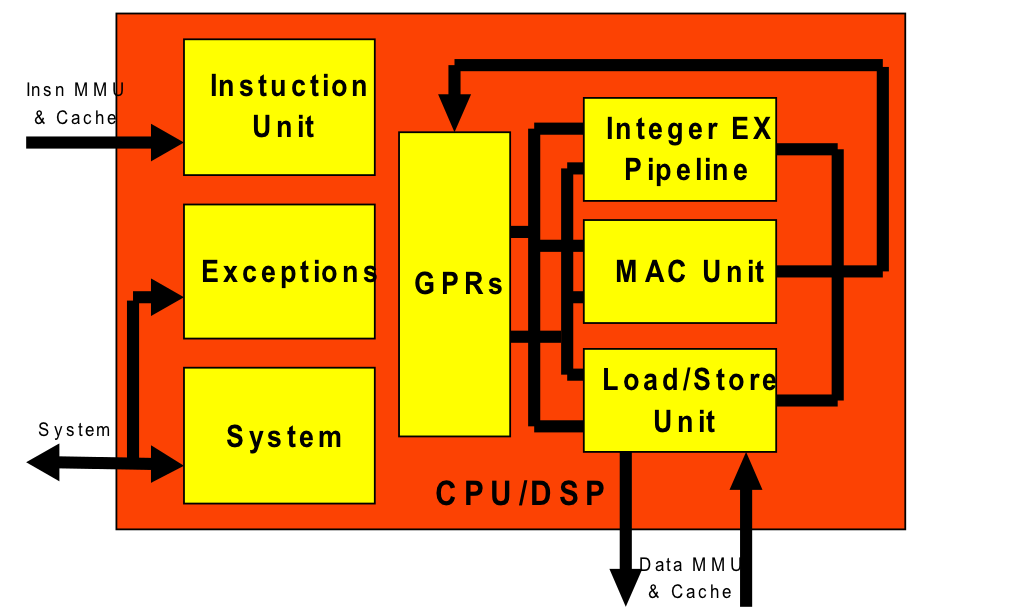
\includegraphics[bb=0 0 1020 613,scale=0.35]{./Images/cpu-dsp.png}
 % cpu-dsp.png: 1020x613 pixel, 72dpi, 35.98x21.63 cm, bb=0 0 1020 613
 \caption{CPU/DSP block diagram.}
\end{figure}

\vspace{0.7cm}

\paragraph{Μονάδα Εντολών\newline\newline}

Η μονάδα εντολών (instruction unit) υλοποιεί την βασική pipeline διαδικασία,φέρνει τις
εντολές απο το υποσύστημα της μνήμης, τις αποστέλει στις διαθέσιμες μονάδες εκτέλεσης (execution unit)
και διατηρεί ενα ιστορικό καταστάσεων ώστε να εξασφαλίσει ένα ακριβές μοντέλο εξαιρέσεων (exception model)
για τον σωστό τερματισμό των εργασιών.Επίσης εκτελεί τις υπό όρους και άνευ όρων εντολές διακλάδωσης.
\newline

Παράλληλα μπορεί να στείλει διαδοχικές εντολές σε κάθε ρολόι αν η κατάλληλη μονάδα εκτέλεσης
είναι διαθέσιμη.Η μονάδα εκτέλεσης είναι αυτή που πρέπει να διακρίνει αν τα δεδομένα που χρειάζεται
η εντολή είναι διαθέσιμα και να διασφαλίσει ότι καμία άλλη εντολή δεν χρησιμοποιεί εκείνη την
στιγμή τον ίδιο καταχωρητή.
\newline

Τέλος η μονάδα εντολών χειρίζεται μόνο τις εντολές της κλάσης ORBIS32 και κατά επιλογή ένα
υποσύνολο των εντολών ORFPX32. Μερικές εντολές της κλάσης ORFPX32  και όλες οι εντολές
των ORFPX3264 και ORVDX64 δεν υποστηρίζονται ακόμα από τον OR1200. 

\paragraph{Καταχωρητές Γενικού Σκοπού\newline\newline}

Ο OpenRISC 1200 χρησιμοποιεί 32 καταχωρητές γενικού σκοπού (general-purpose registers) των 32 δυαδικών ψηφίων.
Η αρχιτεκτονική του επίσης υποστηρίζει σκιώδη αντίγραφα (shadow copies) του αρχείου καταχωρητών (register file)
ώστε να υλοποιεί γρήγορη εναλλαγή μεταξύ των πλαισίων εργασίας (working contexts), όμως
αυτή η λειτουργία δεν υποστηρίζεται από την παρούσα υλοποίηση του OR1200.
\newline

Ο OR1200 υλοποιεί το αρχείο καταχωρητών γενικού σκοπού σαν δυο σύγχρονες μνήμες διπλής θύρας
με χωρητικότητα 32 λέξεων των 32 bit  ανά λέξη.

\paragraph{Μονάδα Load/Store\newline\newline}

Η μονάδα Load/Store (LSU) μεταφέρει όλα τα δεδομένα μεταξύ των καταχωρητών γενικού σκοπού (GPRs) και τον
επεξεργαστή διαμέσου του εσωτερικού διαύλου επικοινωνίας.Έχει υλοποιηθεί σαν μια ανεξάρτητη μονάδα
εκτέλεσης ώστε οι καθυστερήσεις στο υποσύστημα μνήμης λόγω εξαρτήσεων μεταξύ δεδομένων να
επηρεάζει μόνο την pipeline διαδικασία.
\newline

Τα κυριότερα χαρακτηριστικά της μονάδας Load/Store παρουσιάζονται παρακάτω:


\begin{itemize}
 \item όλες οι εντολές Load/Store είναι υλοποιημένες σε επίπεδο hardware (atomic instructions include)
 \item pipeline λειτουργία
 \item ευθυγραμμισμένες προσπελάσεις στην μνήμη
 \item address entry buffer
\end{itemize}

Όταν κάποια εντολή Load ή Store προορίζεται για εκτέλεση τότε η μονάδα Load/Store (LSU)
διερευνά αν όλα τα τελούμενα είναι διαθέσιμα.Τα τελούμενα που ελέγχει είναι τα παρακάτω:


\begin{itemize}
 \item Οι διευθύνσεις των καταχωρητών που θα χρησιμοποιηθούν.
 \item Τα δεδομένα στους καταχωρητές που προορίζονται για εκτέλεση (store εντολή).
 \item Τα δεδομένα στους καταχωρητές που προορίζονται για αποθήκευση (load εντολή).
\end{itemize}

\paragraph{Πράξεις ακεραίων\newline\newline}

Ο πυρήνας του OR1200 υποστηρίζει τα παρακάτω είδη εντολών για πράξεις μεταξύ 32 bit ακεραίων (integer execution pipeline):
\begin{itemize}
 \item Αριθμητικές εντολές.
 \item Εντολές σύγκρισης.
 \item Λογικές εντολές.
 \item Εντολές ολίσθησης και περιστροφής.
\end{itemize}


Οι περισσότερες εντολές μπορούν να εκτελεστούν σε ένα κύκλο(TODO).


\paragraph{Μονάδα MAC\newline\newline}

Η μονάδα MAC εκτελεί λειτουργίες DSP MAC.Οι MAC λειτουργίες είναι 32x32 με 48 bit συσσωρευτή.Η μονάδα MAC είναι υλοποιημένη με την 
τεχνική pipeline και μπορεί να δεχτεί καινούργιες MAC εργασίες σε κάθε καινούργιο κύκλο.

\paragraph{Μονάδα Κινητής Υποδιαστολής\newline\newline}

Η υλοποίηση της μονάδας Κινητής Υποδιαστολής(FPU) είναι βασισμένη σε δύο άλλες FPUs που 
παρέχονται από το OpenCores.org. Για τις συναρτήσεις σύγκρισης και μετατροπής κομμάτια υλοποίησης
έχουν παρθεί απο την FPU που έχει σχεδιαστεί απο τον Rudolf Usselmann, ενώ για τις αριθμητικές
λειτουργίες απο το πρότζεκτ fpu100 όπου ο Jidan Al-Eryani τις μετέτρεψε σε γλώσσα Verilog HDL.


Όλες οι εντολές ORFPX32 εκτός από τις \emph{lf.madd.s} και \emph{lf.rem.s} υποστηρίζονται από την FPU όταν
αυτή έχει ενεργοποιηθεί από τις ρυθμίσεις του OR1200.

\paragraph{Μονάδα Συστήματος\newline\newline}

Η μονάδα συστήματος συνδέει όλα τα σήματα της CPU/FPU/DSP μονάδας που δεν είναι συνδεδεμένα
με τις διεπαφές (interfaces) των εντολών και των δεδομένων.Παράλληλα υλοποιεί όλους τους καταχωρητές ειδικού σκοπού (π.χ. supervisor registers).

\paragraph{Μονάδα Εξαιρέσεων \newline\newline}

Οι εξαιρέσεις του πυρήνα μπορούν να δημιουργηθούν όταν μια συνθήκη εξαίρεσης παρουσιάζεται.Παρακάτω φαίνονται ποιες είναι αυτές
οι συνθήκες για τον OR1200.

\begin{itemize}
 \item Εξωτερικά αιτήματα διακοπών (external interrupt request).
 \item Ορισμένες συνθήκες πρόσβασης στην μνήμη.
 \item Εσωτερικά λάθοι όπως η προσπάθεια εκτέλεσης μη υλοποιημένης εντολής (undefined opcode).
 \item Εσωτερικές εξαιρέσεις όπως σημεία διακοπής (breakpoints).
\end{itemize}

Η μονάδα διαχείρισης εξαιρέσεων είναι αόρατη από το λογισμικό του χρήστη και χρησιμοποιεί τον ίδιο
μηχανισμό για να εξυπηρετεί όλα τα είδη των εξαιρέσεων. Όταν μία εξαίρεση παρουσιάζεται τότε ο έλεγχος
μεταφέρεται στον διαχειριστή εξαιρέσεων με μία προκαθορισμένη μετατόπιση ανάλογα με το είδος της εξαίρεσης που παρουσιάστηκε.
Οι εξαιρέσεις διαχειρίζονται από το supervisor mode.

\subsubsection{Κρυφή Μνήμη Δεδομένων}

Η προκαθορισμένες ρυθμίσεις για την κρυφή μνήμη δεδομένων για τον OR1200 είναι 8-KByte, 1-τρόπων πλήρους απεικόνισης (1-way direct-mapped),
οι οποίες επιτρέπουν στον πυρήνα ταχεία προσπέλαση των δεδομένων.Παρόλα αυτά η κρυφή μνήμη μπορεί να παραμετροποιηθεί σύμφωνα με τον Πίνακα (TODO).
\setlength{\tabcolsep}{3em}
{%
\vspace{0.7cm}
\newcommand{\mc}[3]{\multicolumn{#1}{#2}{#3}}
\definecolor{tcA}{rgb}{1,1,0}
\begin{table}[h]
\begin{center}
\begin{tabular}{ |r|c|}
% use packages: color,colortbl
\hline
\rowcolor{tcA}
  & Direct mapped\\ \hline 
16B/line, 256 lines, 1 way & \mc{1}{c|}{4KB}\\
16B/line, 512 lines, 1 way & \mc{1}{c|}{\textbf{8KB (default)}}\\
16B/line, 1024 lines, 1 way & \mc{1}{c|}{16KB}\\
32B/line, 1024 lines, 1 way & \mc{1}{c|}{32KB} \\ \hline
\end{tabular}
\end{center}
\caption{Ρυθμίσεις μεγέθους κρυφής μνήμης δεδομένων}
\end{table}
\vspace{0.7cm}
}%
\newpage


Ο OR1200  παρέχει την δυνατότητα η κρυφή μνήμη δεδομένων να χρησιμοποιεί είτε την write-through
είτε την write-back στρατηγική, όμως η write-back στρατηγική είναι ακόμα σε πειραματικό στάδιο.
\newline

Χαρακτηριστικά:


\begin{itemize}
 \item Η κρυφή μνήμη δεδομένων είναι ξεχωριστά υλοποιημένη από την κρυφή μνήμη εντολών (Harvard αρχιτεκτονίκη)
 \item Η κρυφή μνήμη δεδομένων χρησιμοποιεί τον αλγόριθμο "Λιγότερο Πρόσφατα Χρησιμοποιημένο" για την αντικατάσταση των πλαισίων.
 \item Ο κατάλογος της κρυφής μνήμης είναι φυσικά διευθυνσιοδοτημένος (physically addressed).Η ετικέτα της φυσικής διεύθυνσης είναι αποθηκευμένη στον κατάλογο της κρυφής μνήμης.
 \item Write-through ή write-back στρατηγική.
 \item Ολόκληρη η κρυφή μνήμη μπορεί να απενεργοποιηθεί, γραμμές να ακυρωθούν, να καθαριστού ή να
γραφτούν πίσω, γράφοντας στους καταχωρητές ειδικού σκοπού της κρυφής μνήμης.
\end{itemize}



Κατά την αστοχία της κρυφής μνήμης και με τις κατάλληλες συνθήκες, η γραμμή της κρυφής μνήμης
γεμίζει ή αδειάζει (written back στρατηγική) με ριπές (burst) των 16-byte.Οι ριπές πραγματοποιούνται
σαν κρίσιμη-λέξη-πρώτα (critical-word-first) λειτουργία˙ η κρίσιμη γράφεται στην κρυφή μνήμη
και ταυτόχρονα προωθείται στην μονάδα αιτήσεων (requesting unit), έτσι μειώνονται οι καθυστερήσεις
που προκαλούνται από το γέμισμα της γραμμής.Η κρυφή μνήμη παρέχει αποθηκευτικό χώρο για τις
ετικέτες και εκτελεί συναρτήσεις αντικατάστασης γραμμών.
\newline

Η κρυφή μνήμη δεδομένων είναι στενά συνδεδεμένη με μια εξωτερική διεπαφή ώστενα επιτρέπει την αποδοτική
πρόσβαση στον ελεκτή μνήμης.
\newline

Παράλληλα η κρυφή μνήμη δεδομένων προμηθεύει τα δεδομένα στου καταχωρητές γενικού σκοπού διαμέσου
της διεπαφής των 32-bit της μονάδας Load/Store. Η μονάδα Load/Store παρέχει όλη την απαραίτητη λογική για
τον υπολογισμό της αποτελεσματικής διεύθυνσης (effective addresses),την κατάλληλη αλληλουχία
για τις λειτουργίες load/store και χειρίζεται την ευθυγράμμιση των δεδομένων από και 
προς την κρυφή μνήμη δεδομένων.Οι λειτουργίες εγγραφής στην κρυφή μνήμη δεδομένων μπορούν
να γίνουν με βάση το 1 byte, την μισή-λέξη (half-word) ή μια λέξη (word).

\vspace{0.7cm}
\begin{figure}[h!]
 \centering
 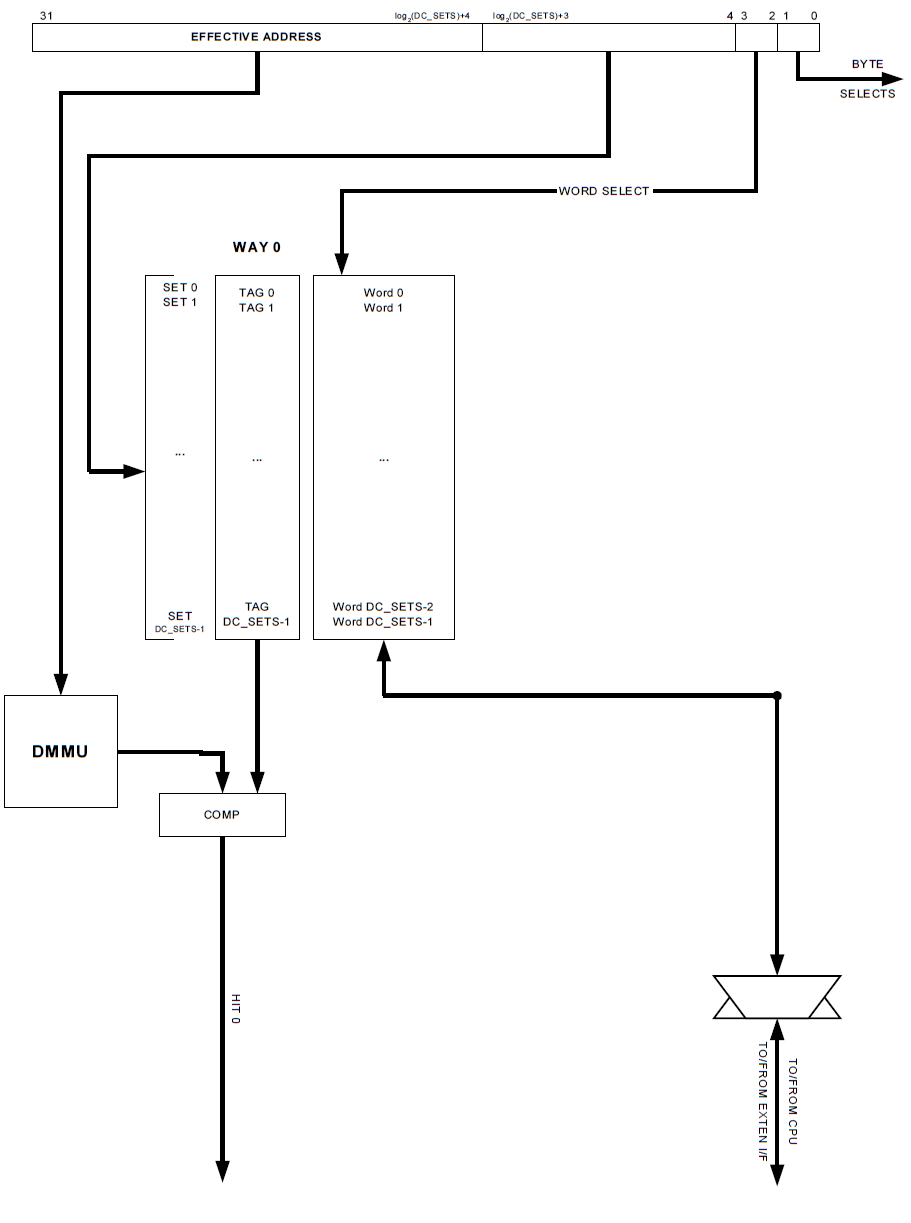
\includegraphics[bb=0 0 906 1228,scale=0.38]{./Images/data_cache.png}
 % data_cache.png: 906x1228 pixel, 72dpi, 31.96x43.32 cm, bb=0 0 906 1228
 \caption{Οργάνωση κρυφής μνήμης δεδομένων.}
\end{figure}
\vspace{0.7cm}

Κάθε γραμμή περιέχει τέσσερις συνεχόμενες λέξεις από τη μνήμη που έχουν φορτωθεί από μια 
οριοθετημένη γραμμή ως προς το μέγεθός της.Ως αποτέλεσμα, οι γραμμές της κρυφής μνήμης 
είναι ευθυγραμμισμένες με τα όρια της σελίδας.

\subsubsection{Κρυφή Μνήμη Εντολών}


Η προκαθορισμένες ρυθμίσεις για την κρυφή μνήμη εντολών για τον OR1200 είναι 8-KByte, 1-τρόπων πλήρους απεικόνισης (1-way direct-mapped),
οι οποίες επιτρέπουν στον πυρήνα ταχεία προσπέλαση στις εντολές.Παρόλα αυτά η κρυφή μνήμη μπορεί να παραμετροποιηθεί σύμφωνα με τον Πίνακα (TODO).
\setlength{\tabcolsep}{3em}
{%
\vspace{0.7cm}
\newcommand{\mc}[3]{\multicolumn{#1}{#2}{#3}}
\definecolor{tcA}{rgb}{1,1,0}
\begin{table}[h]
\begin{center}
\begin{tabular}{ |r|c|}
% use packages: color,colortbl
\hline
\rowcolor{tcA}
  & Direct mapped\\ \hline 
16B/line, 32 lines, 1 way & \mc{1}{c|}{512B}\\
16B/line, 256 lines, 1 way & \mc{1}{c|}{4KB}\\
16B/line, 512 lines, 1 way & \mc{1}{c|}{\textbf{8KB (default)}}\\
16B/line, 1024 lines, 1 way & \mc{1}{c|}{16KB}\\
32B/line, 1024 lines, 1 way & \mc{1}{c|}{32KB} \\ \hline
\end{tabular}
\end{center}
\caption{Ρυθμίσεις μεγέθους κρυφής μνήμης εντολών}
\end{table}
\vspace{0.7cm}
}%


Χαρακτηριστικά:


\begin{itemize}
 \item Η κρυφή μνήμη εντολών είναι ξεχωριστά υλοποιημένη από την κρυφή μνήμη δεδομένων (Harvard αρχιτεκτονίκη).
 \item Η κρυφή μνήμη εντολών χρησιμοποιεί τον αλγόριθμο "Λιγότερο Πρόσφατα Χρησιμοποιημένο" για την αντικατάσταση των πλαισίων.
 \item Ο κατάλογος της κρυφής μνήμης είναι φυσικά διευθυνσιοδοτημένος (physically addressed).Η ετικέτα της φυσικής διεύθυνσης είναι αποθηκευμένη στον κατάλογο της κρυφής μνήμης.
 \item Μπορεί να απενεργοποιηθεί ή να ακυρωθεί/ γράφοντας στους καταχωρητές ειδικού σκοπού της κρυφής μνήμης.
\end{itemize}



Κατά την αστοχία της κρυφής μνήμης η γραμμή της κρυφής μνήμης
γεμίζει ή με ριπές (burst) των 16-byte.Οι ριπές πραγματοποιούνται
σαν κρίσιμη-λέξη-πρώτα (critical-word-first) λειτουργία˙ η κρίσιμη γράφεται στην κρυφή μνήμη
και ταυτόχρονα προωθείται στην μονάδα αιτήσεων (requesting unit), έτσι μειώνονται οι καθυστερήσεις
που προκαλούνται από το γέμισμα της γραμμής.Η κρυφή μνήμη εντολών παρέχει αποθηκευτικό χώρο για τις
ετικέτες και εκτελεί συναρτήσεις αντικατάστασης γραμμών.
\newline

Η κρυφή μνήμη εντολών είναι στενά συνδεδεμένη με μια εξωτερική διεπαφή ώστενα επιτρέπει την αποδοτική
πρόσβαση στον ελεκτή μνήμης.
\newline

Παράλληλα η κρυφή μνήμη εντολών προμηθεύει τις εντολές προς εκτέλεση διαμέσου
της διεπαφής των 32-bit της υπομονάδας προσκόμισης εντολών. Η υπομονάδα προσκόμισης εντολών
 παρέχει όλη την απαραίτητη λογική για
τον υπολογισμό της αποτελεσματικής διεύθυνσης (effective addresses).

\vspace{0.7cm}
\begin{figure}[h!]
 \centering
 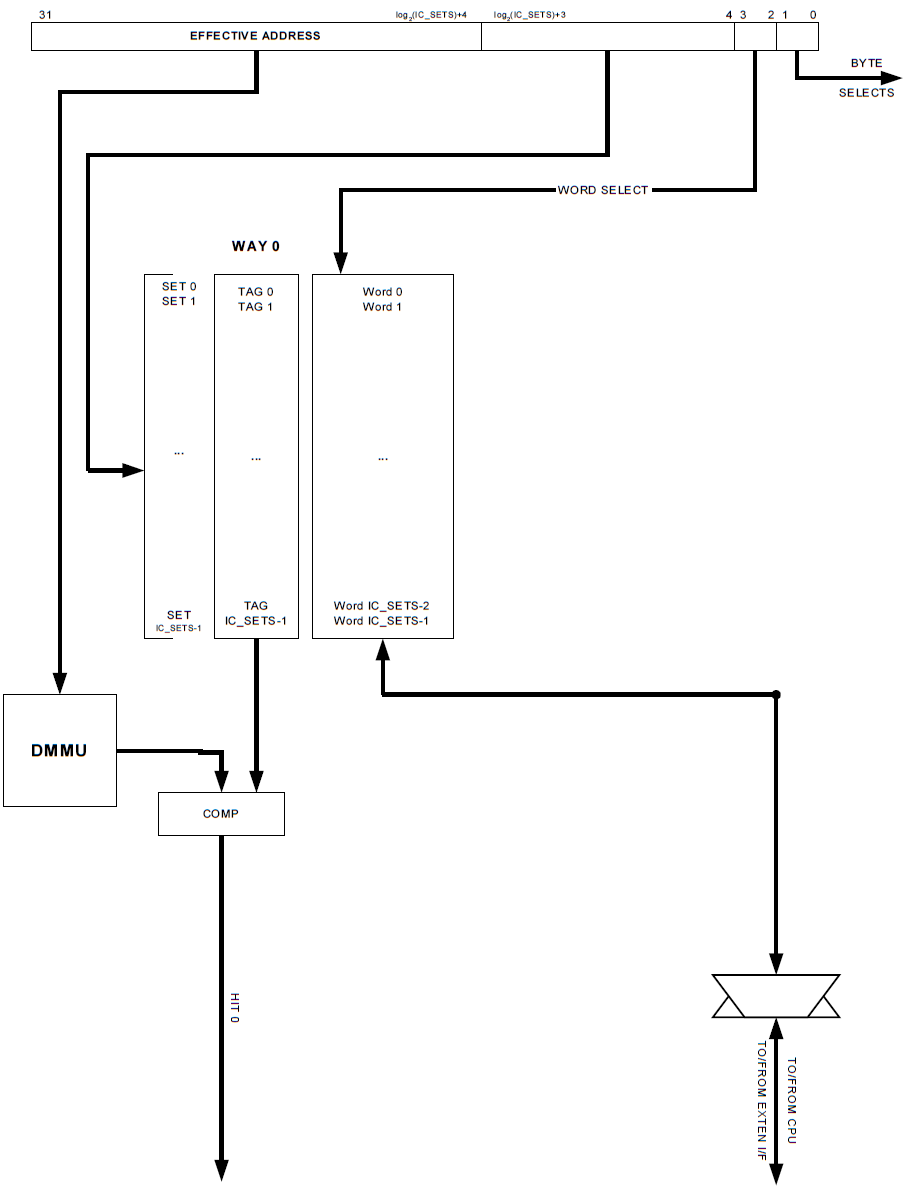
\includegraphics[bb=0 0 908 1201,scale=0.38]{./Images/instruction_cache.png}
 % instruction_cache.png: 908x1201 pixel, 72dpi, 42.37x32.03 cm, bb=0 0 1201 908
 \caption{Οργάνωση κρυφής μνήμης εντολών}
\end{figure}
\vspace{0.7cm}



Κάθε γραμμή περιέχει τέσσερις συνεχόμενες λέξεις από τη μνήμη που έχουν φορτωθεί από μια 
οριοθετημένη γραμμή ως προς το μέγεθός της.Ως αποτέλεσμα, οι γραμμές της κρυφής μνήμης 
είναι ευθυγραμμισμένες με τα όρια της σελίδας.

\subsubsection{Διαχείριση Μνήμης (MMU) Δεδομένων}

Η OR1200 υλοποιεί ένα εικονικό σύστημα διαχείρισης μνήμης (memomy management unit - MMU) 
που παρέχει προστασία κατά την πρόσβαση στην μνήμη και αποτελεσματική μετάφραση σε φυσικές
 διευθύνσεις. Η διακριτότητα της προστασίας είναι όπως ορίζεται από την αρχιτεκτονίκη 
OpenRISC 1000 8-Kbyte και 16-Mbyte σελίδες.

\setlength{\tabcolsep}{3em}
{%
\vspace{0.7cm}
\newcommand{\mc}[3]{\multicolumn{#1}{#2}{#3}}
\definecolor{tcA}{rgb}{1,1,0}
\begin{table}[h]
\begin{center}
\begin{tabular}{ |r|c|}
% use packages: color,colortbl
\hline
\rowcolor{tcA}
  & Direct mapped\\ \hline 
16 entries per way & \mc{1}{c|}{16 DTLB entries}\\
32 entries per way& \mc{1}{c|}{32 DTLB entries}\\
64 entries per way & \mc{1}{c|}{\textbf{64 DTLB entries (default)}}\\
128 entries per way & \mc{1}{c|}{128 DTLB entries} \\ \hline
\end{tabular}
\end{center}
\caption{Ρυθμίσεις Δεδομένων TLB (translation lookaside buffer)}
\end{table}
\vspace{0.7cm}
}%


Χαρακτηριστικά:

\begin{itemize}
 \item H MMU δεδομένων είναι ξεχωριστή από την MMU εντόλων.
 \item Το μέγεθός της σελίδας είναι 8-KByte.
 \item Ολοκληρωμένο σύστημα προστασίας σελίδας.
 \item Πλήρης απεικόνιση κατακερματισμού βασισμένο στον translation lookaside buffer (DTLB)
με προκαθορισμένο 1-τροπο συσχέτισης και τα παρακάτω χαρακτηριστικά:
	  \begin{itemize}
	      \item Παροχή εξαιρέσεων στην περίπτωση εξαιρέσεων και λαθών.
	      \item Software tablewalk.
	      \item Υψηλή απόδοση λόγο του κατακερματισμού.
	      \item Τροποποιήσιμο αριθμό καταχωρήσεων στο DLTB με προκαθορισμένες τις 64 καταχωρήσεις ανά τρόπο.
	  \end{itemize}
\end{itemize}

\newpage
\vspace{0.7cm}
\begin{figure}[h!]
 \centering
 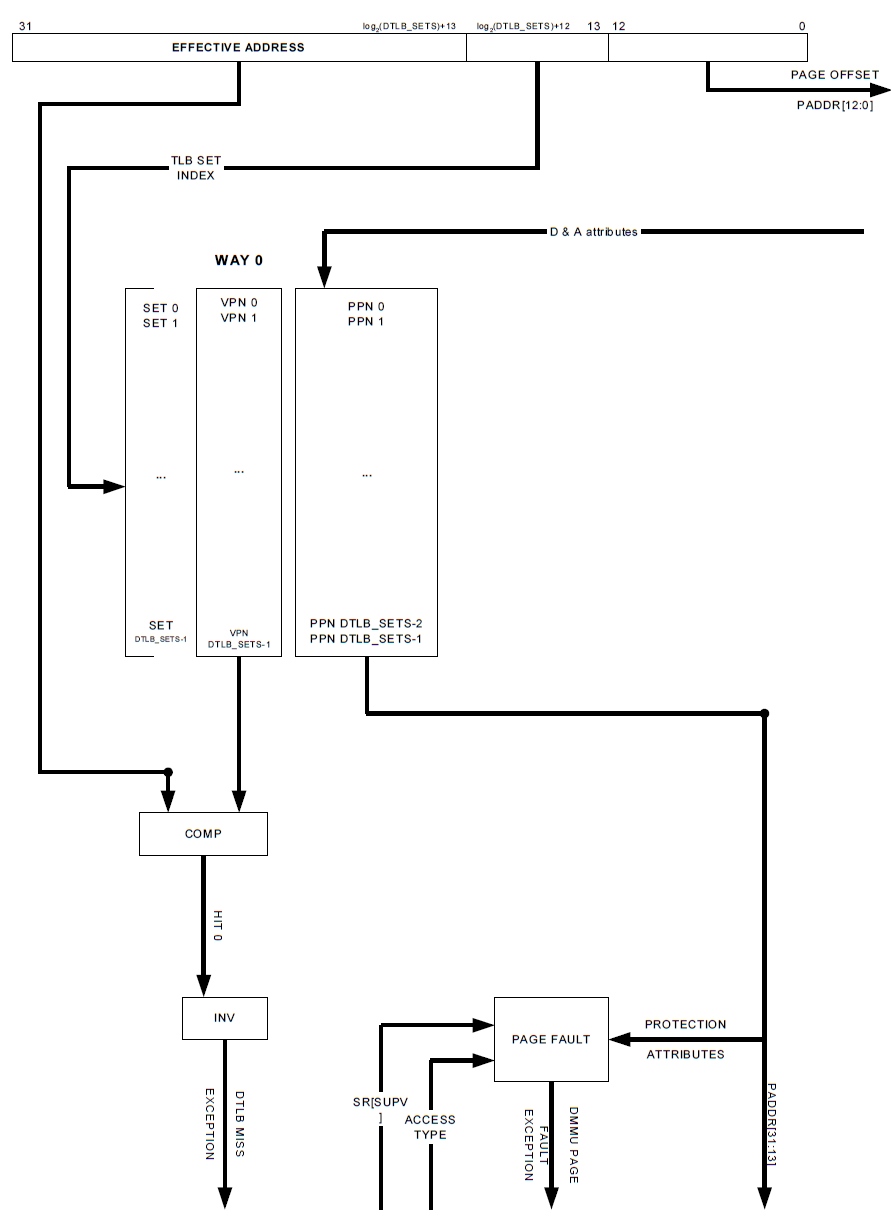
\includegraphics[bb=0 0 891 1229,scale=0.38]{./Images/data_MMU.png}
 % data_MMU.png: 891x1229 pixel, 72dpi, 31.43x43.36 cm, bb=0 0 891 1229
 \caption{Οργάνωση MMU δεδομένων.}
\end{figure}
\vspace{0.7cm}

Η υλοποίηση της MMU σε υλικό υποστηρίζει δύο-επιπέδων software tablewalk.

\subsubsection{Διαχείριση Μνήμης (MMU) Εντολών}

Η OR1200 υλοποιεί ένα εικονικό σύστημα διαχείρισης μνήμης (memomy management unit - MMU) 
που παρέχει προστασία κατά την πρόσβαση στην μνήμη και αποτελεσματική μετάφραση σε φυσικές
 διευθύνσεις. Η διακριτότητα της προστασίας είναι όπως ορίζεται από την αρχιτεκτονίκη 
OpenRISC 1000 8-Kbyte και 16-Mbyte σελίδες.

\setlength{\tabcolsep}{3em}
{%
\vspace{0.7cm}
\newcommand{\mc}[3]{\multicolumn{#1}{#2}{#3}}
\definecolor{tcA}{rgb}{1,1,0}
\begin{table}[h]
\begin{center}
\begin{tabular}{ |r|c|}
% use packages: color,colortbl
\hline
\rowcolor{tcA}
  & Direct mapped\\ \hline 
16 entries per way & \mc{1}{c|}{16 ΙTLB entries}\\
32 entries per way& \mc{1}{c|}{32 ΙTLB entries}\\
64 entries per way & \mc{1}{c|}{\textbf{64 ΙTLB entries (default)}}\\
128 entries per way & \mc{1}{c|}{128 ΙTLB entries} \\ \hline
\end{tabular}
\end{center}
\caption{Ρυθμίσεις Εντολών TLB (translation lookaside buffer)}
\end{table}
\vspace{0.7cm}
}%


Χαρακτηριστικά:

\begin{itemize}
 \item H MMU εντόλων είναι ξεχωριστή από την MMU δεδομένων.
 \item Το μέγεθός της σελίδας είναι 8-KByte.
 \item Ολοκληρωμένο σύστημα προστασίας σελίδας.
 \item Πλήρης απεικόνιση κατακερματισμού βασισμένο στον translation lookaside buffer (ΙTLB)
με προκαθορισμένο 1-τροπο συσχέτισης και τα παρακάτω χαρακτηριστικά:
	  \begin{itemize}
	      \item Παροχή εξαιρέσεων στην περίπτωση εξαιρέσεων και λαθών.
	      \item Software tablewalk.
	      \item Υψηλή απόδοση λόγο του κατακερματισμού.
	      \item Τροποποιήσιμο αριθμό καταχωρήσεων στο ILTB με προκαθορισμένες τις 64 καταχωρήσεις ανά τρόπο.
	  \end{itemize}
\end{itemize}

\newpage
\vspace{0.7cm}
\begin{figure}[h!]
 \centering
 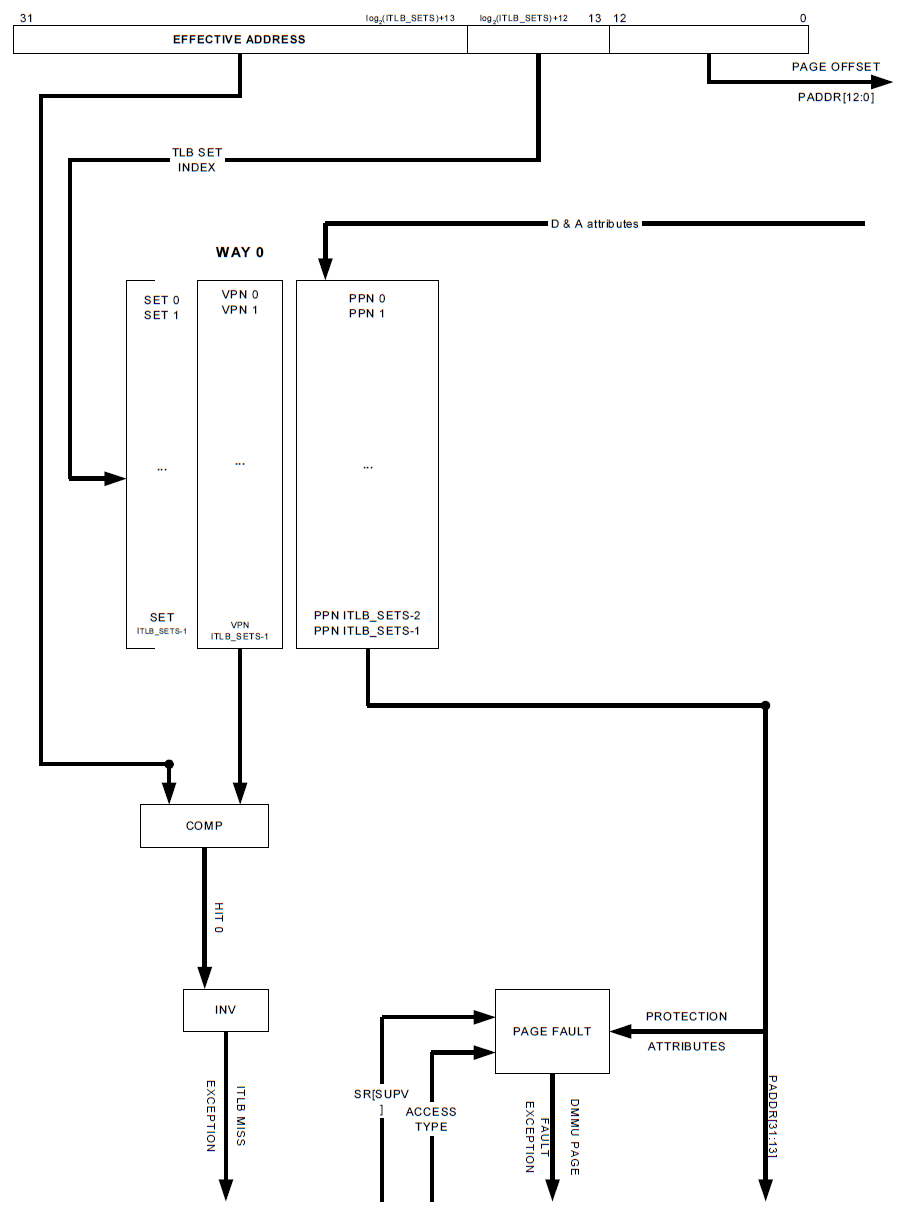
\includegraphics[bb=0 0 891 1229,scale=0.38]{./Images/instruction_MMU.png}
 % data_MMU.png: 891x1229 pixel, 72dpi, 31.43x43.36 cm, bb=0 0 891 1229
 \caption{Οργάνωση MMU εντολών.}
\end{figure}
\vspace{0.7cm}

Η υλοποίηση της MMU σε υλικό υποστηρίζει δύο-επιπέδων software tablewalk.

\subsubsection{Προγραμματιζόμενος Ελεγκτής Διακοπών}

Ο ελεγκτής διακοπών (Interrupt controller) λαμβάνει διακοπές από εξωτερικές πηγές και τις
προωθεί ανάλογα με την προτεραιότητά τους (χαμηλή-υψηλή) σαν εξαιρέσεις (exception) στον
πυρήνα του επεξεργαστή.

\vspace{0.7cm}
\begin{figure}[h!]
 \centering
 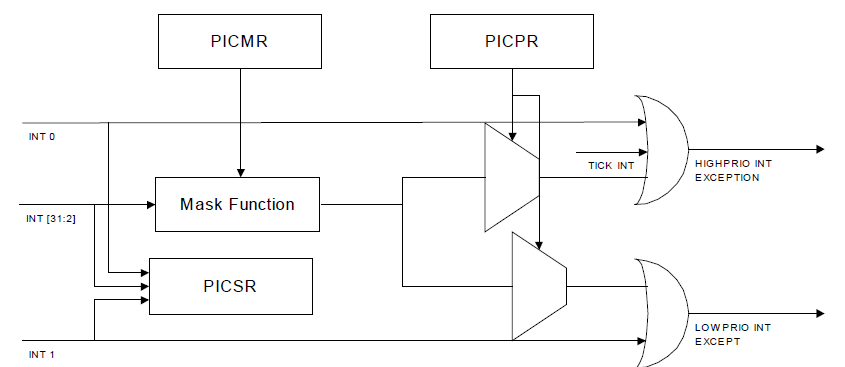
\includegraphics[bb=0 0 845 367,scale=0.38]{./Images/inter_controller.png}
 % inter_controller.png: 845x367 pixel, 72dpi, 29.81x12.95 cm, bb=0 0 845 367
 \caption{Μπλοκ διάγραμμα του ελεγκτή διακοπών.}
\end{figure}
\vspace{0.7cm}


Ο προγραμματιζόμενος ελεγκτής διακοπών έχει τρεις καταχωρητές ειδικού σκοπού και 32 
σήματα εισόδου διακοπών.Τα σήματα εισόδου διακοπών 0 και 1 είναι πάντα ενεργοποιημένα και συνδεδεμένα 
με την υψηλή και την χαμηλή προτεραιότητα εισόδου ​​αντίστοιχα, όπως φαίνεται και στο σχήμα (TODO).
\newline

Υπάρχουν 30 ακόμα σήματα εισόδου που μπορούν να φιλτράριστουν και να ανατεθεί προτεραιότητά 
διαμέσου του προγραμματισμού των καταχωρητών ειδικού σκοπού.

\subsubsection{Tick Timer}

O επεξεργαστής OR1200 έχει υλοποιημένη λειτουργία χρονιστή (tick timer).Βασικά αυτός είναι
ένας χρονοδιακόπτης που χρονίζεται από το ρολόι του επεξεργαστή και χρησιμοποιείται από το
λειτουργικό σύστημα για ακριβείς μετρήσεις χρόνου και για τον χρονοπρογραμματισμό των διεργασιών τους
συστήματος.
\newline

Ο OR1200 ακολουθεί αυστηρά τον αρχιτεκτονικό ορισμό του χρονιστή όπου:

\begin{itemize}
 \item Μέγιστες μετρήσεις του χρονιστή $2^{32}$ κύκλους ρολογιού.
 \item Μέγιστη χρονική περίοδο, $2^{28}$ κύκλους ρολογιού μεταξύ διακοπών.
 \item Φιλτραρισμένο σήμα διακοπής χρονιστή (Maskable tick timer interrupt).
 \item Δυνατότητα επανεκκίνησης, μονής και συνεχούς μέτρησης.
\end{itemize}


\subsubsection{Διαχείριση Ενεργειακών Απαιτήσεων}

Για την βελτιστοποίηση της κατανάλωσης ενέργειας, ο OR1200 παρέχει καταστάσεις (mode)
χαμηλής ενεργειακής κατανάλωσης που μπορούν να χρησιμοποιηθούν ώστε δυναμικά να ενεργοποιούνται
και να απενεργοποιούνται ορισμένες εσωτερικές ενότητες (module).
\newline

Ο OR1200 έχει τρεις κύριες λειτουργίες για την ελαχιστοποίηση της κατανάλωσης ενέργειας:
\begin{itemize}
 \item Slow και Idle καταστάσεις (SW controlled clock freq reduction)
 \item Doze και Sleep καταστάσεις (interrupt wake-up)
\end{itemize}

\setlength{\tabcolsep}{1em}
\definecolor{tcA}{rgb}{1,1,0}
\begin{table}[h]
\begin{center}
\begin{tabular}{|l|l|}\hline
% use packages: color,colortbl
\rowcolor{tcA}
Power Minimization Feature & Approx Power Consumption Reduction\\\hline
Slow and Idle mode & 2x – 10x\\\hline
Doze mode & 100x\\\hline
Sleep mode & 200x\\\hline
Dynamic clock gating & N/A\\\hline
\end{tabular}
\end{center}
\caption{Καταστάσεις βελτιστοποίησης κατανάλωσης ενέργειας.}
\end{table}


Η κατάσταση Slow Down εκμεταλλεύεται τους low-power διαιρέτες από το εξωτερικό κύκλωμα 
παραγωγής ρολογιού ώστε να επιτυγχάνει πλήρης λειτουργικότητα αλλά σε χαμηλότερη συχνότητα,
εξοικονομώντας έτσι ενέργεια.
\newline

Όταν το λογισμικό εκκινεί την κατάσταση Doze, τότε τα προγράμματα που τρέχουν στον επεξεργαστή
αναστέλλονται.Τα ρολόγια στις εσωτερικές ενότητες (modules) του επεξεργαστή απενεργοποιούνται 
εκτός του χρονιστή (tick timer). Ωστόσο οποιοδήποτε αλλό μπλόκ πάνω στο ολοκληρωμένο κύκλωμα
συνεχίζει να λειτουργέι κανονικά.Ο επεξεργαστής OR1200 θα φύγει από την κατάσταση doze και 
θα επανέλθει σε κανόνική κατάσταση όταν κάποια διακοπή (interrupt) παρουσιαστεί.
\newline

Στην κατάσταση Sleep, όλες οι εσωτερικές μονάδες του OR1200 απενεργοποιούνται και τα 
ρολόγια οριοθετούνται (clocks gated).Προαιρετικά (ανάλογα με την υλοποίηση) μπορεί να χαμηλωθεί 
η παροχή της τάσης στον πυρήνα του OR1200. επεξεργαστής OR1200 θα φύγει από την κατάσταση doze και 
θα επανέλθει σε κανόνική κατάσταση όταν κάποια διακοπή (interrupt) παρουσιαστεί.
\newline

Η λειτουργία Dynamic Clock gating δεν υποστηρίζεται προς το παρών από τον OR1200. 

\subsubsection{Μονάδα Αποσφαλμάτωσης}

Η μονάδα αποσφαλμάτωσης βοηθάει τους προγραμματιστές λογισμικού διορθώσουν λάθοι στο σύστημα
τους.Παρέχει την βασική βοήθεια για αποσφαλμάτωση, χωρίς να παρέχει όμως προηγμένη τεχνολογία
σύμφωνα με την αρχιτεκτονίκη του OpenRISC 1000 όπως watchpoints, breakpoints και πρόγραμμα
ελέγχου της ροής των καταχωρητών ελέγχου.

\vspace{0.7cm}
\begin{figure}[h!]
 \centering
 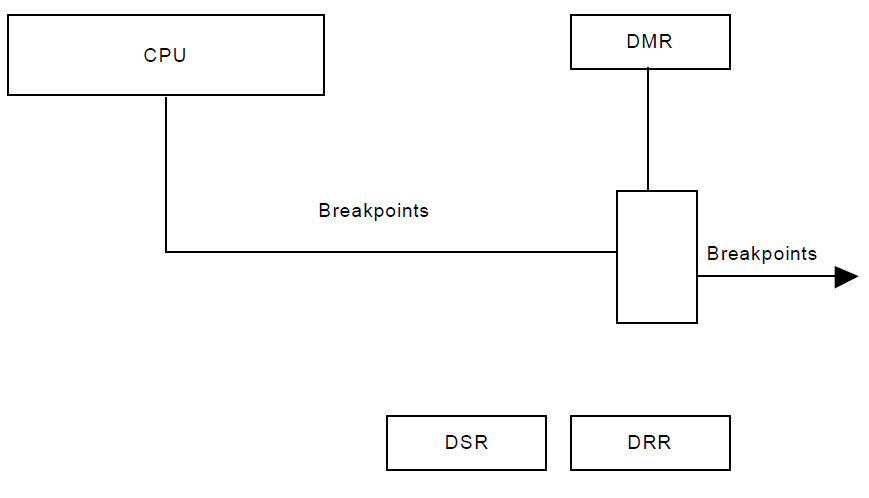
\includegraphics[bb=0 0 869 498,scale=0.38]{./Images/debug_unit.png}
 % debug_unit.png: 869x498 pixel, 72dpi, 30.66x17.57 cm, bb=0 0 869 498
 \caption{Μπλόκ διάγραμμα μονάδας αποσφαλμάτωσης.}
\end{figure}
\vspace{0.7cm}

\subsubsection{Σήματα Χρονισμού και Επανεκκίνησης}
(TODO)
O πυρήνας του OR1200 χρησιμοποιεί ένα ρολόι για τον χρονισμό κάθε μιας διεπαφή του διαύλου
επικοινωνίας Wishbone τόσο για τα δεδομένα όσο και για τις εντολές.Το σήμα ρολογιού \emph{clk\_cpu}
χρονίζει οτιδήποτε βρίσκεται μέσα στην διεπαφή του διαύλου Wishbone.Η διεπαφή διαύλου δεδομένων
Wishbone χρονίζεται από το σήμα \emph{dwd\_clk\_i}, ενώ των εντολών με το σήμα \emph{iwd\_clk\_i}.
\newline

O επεξεργαστής OR1200 παρέχει ένα ασύγχρονο σήμα επανεκκίνησης του συστήματος (asynchronous reset signal)
,\emph{rst}. Όταν αυτό σήμα είναι ενεργοποιημένο τότε αμέσως επαναφέρει (resets) όλα τα 
flip-flops μέσα στον OR1200.Όταν είναι απενεργοποιημένο τότε ο επεξεργαστής λειτουργεί κανονικά.

\subsubsection{Δίαυλος επικοινωνίας Wishbone}

Δύο διεπαφές Wishbone του επεξεργαστή OR1200 συνδέουν τον πυρήνα με τα περιφερειακά και το
εξωτερικό υποσύστημα μνήμης.Αυτές είναι συμβατές το WISHBONE SoC Interconnection specification Rev. B3.
Η υλοποίηση παρέχει ένα δίαυλο επικοινωνίας πλάτους 32 bit χωρίς να υποστηρίζει άλλα πλάτη.

(TODO)

\newpage
}



\section{OR1200 Simulation}{

\subsection{Simulation Enviroment}{
Υπάρχουν δύο περιβάλλοντα με τα οποία γίνετε η εξομοίωση του OR1200 επεξεργαστή.
Το πρώτο χρησιμοποιεί τον OpenRISC αρχιτεκτονικό εξομοιωτή \emph{or1ksim} και 
το δεύτερο χρησιμοποιεί τον \emph{NC-Verilog} εξoμοιωτή που κάνει εξομοίωση με βάση
το υλικό (hardware based simulation).Στο πρώτο περιβάλλον γίνετε η επαλήθευση
της λειτουργικότητας των benchmarks και στο δεύτερο προσομοιώνεται η ουσιαστική
λειτουργία του OR1200 σε επίπεδο υλικού με βάση το benchmark που εκτελέσαμε.\newline


Η συνολική ροή της εξομοίωσης παρουσιάζεται στο Σχήμα 4.Τα benchmarks είναι 
είτε .C αρχέια είτε .S αρχεία.Αυτά τα αρχεία, αρχίκα γίνονται cross-compiled
 χρησιμοποιώντας την εντολή or32-uclinux-gcc και παράγουν ένα .O object αρχείο.
Το object αρχείο μετά μετατρέπεται σε ενα .OR32 εκτελέσιμο αρχείο χρησιμοποιώντας
την συνδετική εντολή or32-uclinux-ld. Αυτό το εκτελέσιμο αρχέιο χρησιμοποιείται
απο τον or1k αρχιτεκτονικό εξομοιωτή.Περαιτέρω το αρχείο .OR32 μετατρέπεται σε
δυαδικό (binary) αρχείο χρησιμοποιώντας την εντολή or32-uclinux-objcopy.Στο τέλος
δημιουργείται ενα .HEX αρχείο χρησιμοποιώντας τον binary to hex μετατροπέα
 bin2hex. Το παραγώμενο αρχείο .HEX φορτώνεται στην flash μνημη του RTL κώδικα
του OR1200 επεξεργαστή και μετά γινετε η εξομοίωση με βάση το υλικό.
 
\begin{figure}[h!]
 \centering
 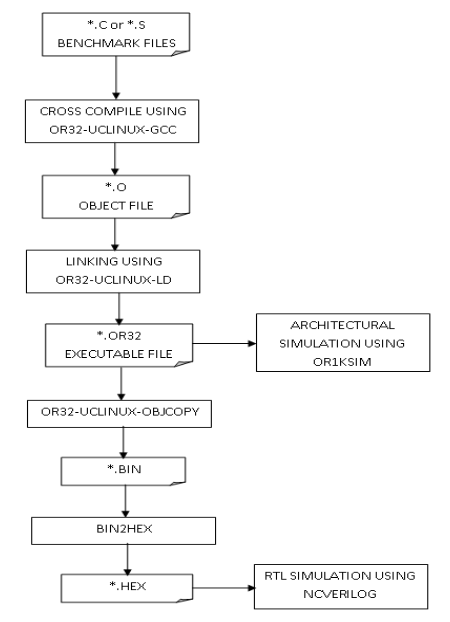
\includegraphics[bb=0 0 450 622,scale=0.5]{/home/federico/Documents/Kile/Diploma/Images/overall_flow.png}
 % overall_flow.png: 450x622 pixel, 72dpi, 15.88x21.94 cm, bb=0 0 450 622
 \caption{Συνολική ροή εξομοίωσης.}
\end{figure}


}



\subsection{Package Structure}{
Σε αυτό το μέρος θα παρουσιάσουμε την δομή και τα περιεχομενα του φακέλου που αποτελεί 
τον επεξεργαστή OR1200.

Το συγκεκριμένο πακέτο περιέχει:
\begin{itemize}
 \item \underline{{\bf Rtl}} : Εδώ βρίσκεται ο κώδικας verilog που περιγράφει σε υλικό τον επεξεργαστή OR 1200.
\item \underline{{\bf Boards}} : Περιέχει κατάλληλα αρχεία για να περάσεις τον OR1200 σε συγκεκριμένες πλακετες
FPGA.
\item \underline{{\bf Sim}} : Σε αυτό τον φάκελο δημιουργούνται τα αποτελέσματα της εξομοίωσης σύμφωνα με
το Makefile που δημιουργήσαμε για τους σκοπούς του εργαστηρίου. \begin{enumerate}
                                                                 \item \emph{sim/bin} : Εδώ βρίσκεται το Makefile που δημιουργήσαμε για τους σκοπούς του
εργαστηρίου και χειρίζεται την λειτούργια του επεξεργαστή.
                                                                 \item \emph{sim/run} :Εδώ εκτελούνται όλες οι εντολές που σχετίζονται με την εξομοίωση
του επεξεργαστη.
                                                                 \item \emph{sim/out} :Εδώ τοποθετούνται όλα τα αρχεία που παράγονται μετά την εξομοίωση.
Να σημειωθεί οτι τα waveforms τοποθετούνται στο sim/run.
                                                                \end{enumerate}

\item \underline{{\bf Sw}} : Εδω βρίσκονται τα βασικότερα αρχεία που είναι απαραίτητα για το cross-compilation 
και την σωστή λειτουργία του OpenRISC επεξεργαστή.
					  \begin{enumerate}
                                           \item \emph{sw/drivers} :Εδω βρίσκονται οι drivers και τα εργαλεία για τροποποίηση του hardware.
					   \item \emph{sw/lib} :Eδω βρίσκεται μια απλή βιβλιοθήκη που σε συνδυασμο με τους drivers κατά την διάρκεια του compile δημηιουργούν την βιβλιοθήκη liborpsoc 
που τοποθετείται στο \emph{sw/lib}.
					   \item \emph{sw/lib/include} :Εδώ βρίσκεται το αρχείο cpu-utils.h που περιέχει όλες τις συναρτήσεις σχετίκες
με την CPU του OpenRISC.
					   \item \emph{sw/tests} :Εδώ βρίσκεται το λογισμικό που χρησιμοποιείται (.C και .S αρχέια) για να δοκιμαστεί η σωστή λειτουργία
του επεξεργαστή (testing) σε υπομονάδες οπως ethmac, or1200,sdram, spi και uart.Στον φάκελο κάθε υπομονάδας (πχ sw/test/sdram) υπάρχουν δύο υποφάκελοι board 
και sim (πχ sw/test/sdram/board και sw/test/sdram/sim).Στον sim φάκελο υπαρχουν τα tests που εκτελούνται κατα την εξομοίωση του επεξεργαστη σε ενα PC και στον
φάκελο board υπάρχουν τα tests που εκτελούνται κατά την λειτουργία του επεξεργαστή.
                                          \end{enumerate}

\item \underline{{\bf Doc}} : Εδω βρισκεται documentation που χρειαζόμαστε για να καταλαβουμε την φύση των
testbenches και οι οδηγιες για το simulation συμφωνα με το Makefile που δημιουργησαμε για τους σκοπους του εργαστηρίου.
\end{itemize}
}



\subsection{Simulation commands}{
{
\subsubsection{ Η βασική διαδικασία}
{

Η διαδικασία με την οποία γίνετε η εξομοίωση του OR1200 είναι η εξής:
\begin{enumerate}
 \item Το Makefile που ελέγχει το simulation βρίσκετε στο \emph{/sim/bin/} και είναι προσπελάσιμο και απο το \emph{/sim/run/} .
 \item Στον φάκελο \emph{/sim/run/} εκτελώντας την εντολή \emph{make rtl-tests} κανει compile τον rtl
(verilog) κωδικα του OR1200 και εκτελεί όλα τα testbenches (assembly) που βρίσκονται στο \emph{sw/tests/or1200}.
 \item Tα αποτελέσματα του παραπάνω βήματος τοποθετούνται στο \emph{/sim/out/}. Aυτα ειναι (στα αγγλίκα για καλύτερη κατανόηση):
    \begin{itemize}
     \item \emph{test-name-executed.log} : A trace of the processor after each executed instruction
     \item \emph{test-name-sprs.log} : A list of processor special purpose registers (SPR) accesses is created
     \item \emph{test-name-lookup.log} : A list of when each instruction was executed is generated
     \item \emph{test-name-general.log} : The use of the processor’s report mechanism is commonplace in the
test software, as it allows for the checking of intermediate values after simulation.
    \end{itemize}
\end{enumerate}
}

\subsubsection{ Εκτέλεση ενος συγκεκριμένου test}
{

Η εξομοίωση ενός συγκεκριμένου test γίνετε με την εντολή
\emph{make rtl-test TEST=test-name\footnote{test-name: Είναι η ονομασία του test που θέλουμε να εκτελέσουμε.}} .Πρέπει το αρχείο \emph{test-name.c}
 (ή \emph{test-name.s} )να είναι τοποθετημένο στο \emph{sw/tests/module /sim/ } όπου module ειναι η υπομονάδα που θέλουμε να ελέξουμε με κάποιο απο τα tests που μας παρέχει 
(πχ sw/tests/sdram/sim/sdram-rows.c).
}

\subsubsection{Εκτέλεση συγκεκριμένων tests μαζί}
{

Η εξομοίωση πολλών συγκεκριμένων tests γίνετε με την εντολή \emph{make rtl-test TEST=" test-name1 test-name2 ..."} (πχ make rtl-tests TESTS="sdram-rows uart-simple or1200-mmu or1200-fp")
}


\subsubsection{ Παρέχοντας μια προσαρμοσμένη VMEM εικόνα (image)}
{

Είναι δυνατό να καθορίσουμε το μονοπάτι μιας ήδη υπάρχουσας VMEM εικόνας που θα την
χρησιμοποιήσουμε αντί να κάνουμε πάλι απο την αρχή test το software.Χρησιμοποιώντας
την μεταβλητή \emph{USER\_VMEM} μπορούμε να καθορίσουμε το μονοπάτι της VMEM εικόνας
που θέλουμε να τρέξουμε. Για παράδειγμα \emph{make rtl-test USER\_VMEM=/path/to/myapp.vmem}
Αυτή η εικόνα θα αντιγραφεί στο φάκελο στον οποίο εργαζόμαστε και θα μετονομαστέι
σύμφωνα με το τι η μνήμη στην εξομοίωση απαιτεί.
}

\subsubsection{ Παρέχοντας ένα "precompiled" εκτελέσιμο .ELF αρχέιο}
{

Είναι δυνατό να καθορίσουμε το μονοπάτι ενός OR32 ELF εκτελέσιμου αρχείου που θα το
χρησιμοποιήσουμε αντί να κάνουμε πάλι απο την αρχή test το software.Χρησιμοποιώντας
την μεταβλητή \emph{USER\_ELF} μπορούμε να καθορίσουμε το μονοπάτι στο οποίο βρίσκετε
αυτό το αρχείο. Για παράδειγμα \emph{make rtl-test USER\_ELF=/path/to/myapp.elf}
Το ELF αρχείο θα μετατραπεί σe δυαδίκη μορφή και μετά σε VMEM και θα φορτωθεί στο
μοντέλο για να εκτελεστέι.
}


\subsubsection{ Κυματομορφές}
{

Παράλλημα με το simulation ενός ή περισσοτέρων testbench παράγονται και οι κυματομορφές
των εξομοιώσεων που μας βοηθάνε στην καλύτερη κατανόηση τους.Τα αρχεία που παράγονται
βρίσκονται σε φακέλους μέσα στο \emph{/sim/run/} που έχουν την ονομασία \emph{test-name.shm} .Για να
εμφανίσεις τις κυματομορφές αυτές πρέπει μέσω κονσόλας να οδηγηθείς στο /sim/run/ και
μετά να εκτελέσεις την εντολή \emph{simvision test-name.shm}.
}

\subsubsection{ Eπιπρόσθετα επιλογές στις εντολες}
{

Παρακάτω παρουσιάζονται μερίκες μεταβλητές που μας βοηθούν να επιλέξουμε καποιές
συγκεκριμένες λειτουργίες.
\begin{itemize}
 \item \emph{END\_TIME    :}Αναγκάζει την εξομοίωση να τερματίσει (\$finish).Πχ 
\emph{make rtl-test TEST="or1200-mul" END\_TIME=100} όπου είναι ίδιο με το \emph{\#100 \$finish} σε αρχείο verilog.
\item \emph{DISABLE\_PROCESSOR\_LOGS    :} Απενεργοποιεί την οθόνη παρακολούθησης του επεξεργαστή
που συλλέγει πληροφορίες κατα την εκτέλεση μιας εξομοίωσης .Αυτό βοηθάει στην επιτάχυνση της εξομοίωσης αφού απαιτείται λιγότερος χρόνος στην
εγραφή αρχείων και αποτρέπει την δημιουργία πολύ μεγάλων αρχείων σε χρονοβόρες εξομοιώσεις.
\item \emph{SIMULATOR    :}Επιλέγουμε τον εξομοιωτή υλικου που θέλουμε να χρησιμοποιήσουμε.
Προκαθορισμένος εξομοιωτής ειναι ο NC-Verilog.Άλλη επιλόγη ειναι το ICARUS.
\end{itemize}

}
}
}

\end{document}